\section{Analysis of Different SQL Generators}
\label{sec:exp-gen}


%\begin{wrapfigure}{r}{0.5\linewidth}
%\centering
%\rule{0.9\linewidth}{0.75\linewidth}
%\caption{Dummy figure.}
%\label{fig:myfig}
%\end{wrapfigure}
%\blindtext

\begin{figure}
\centering
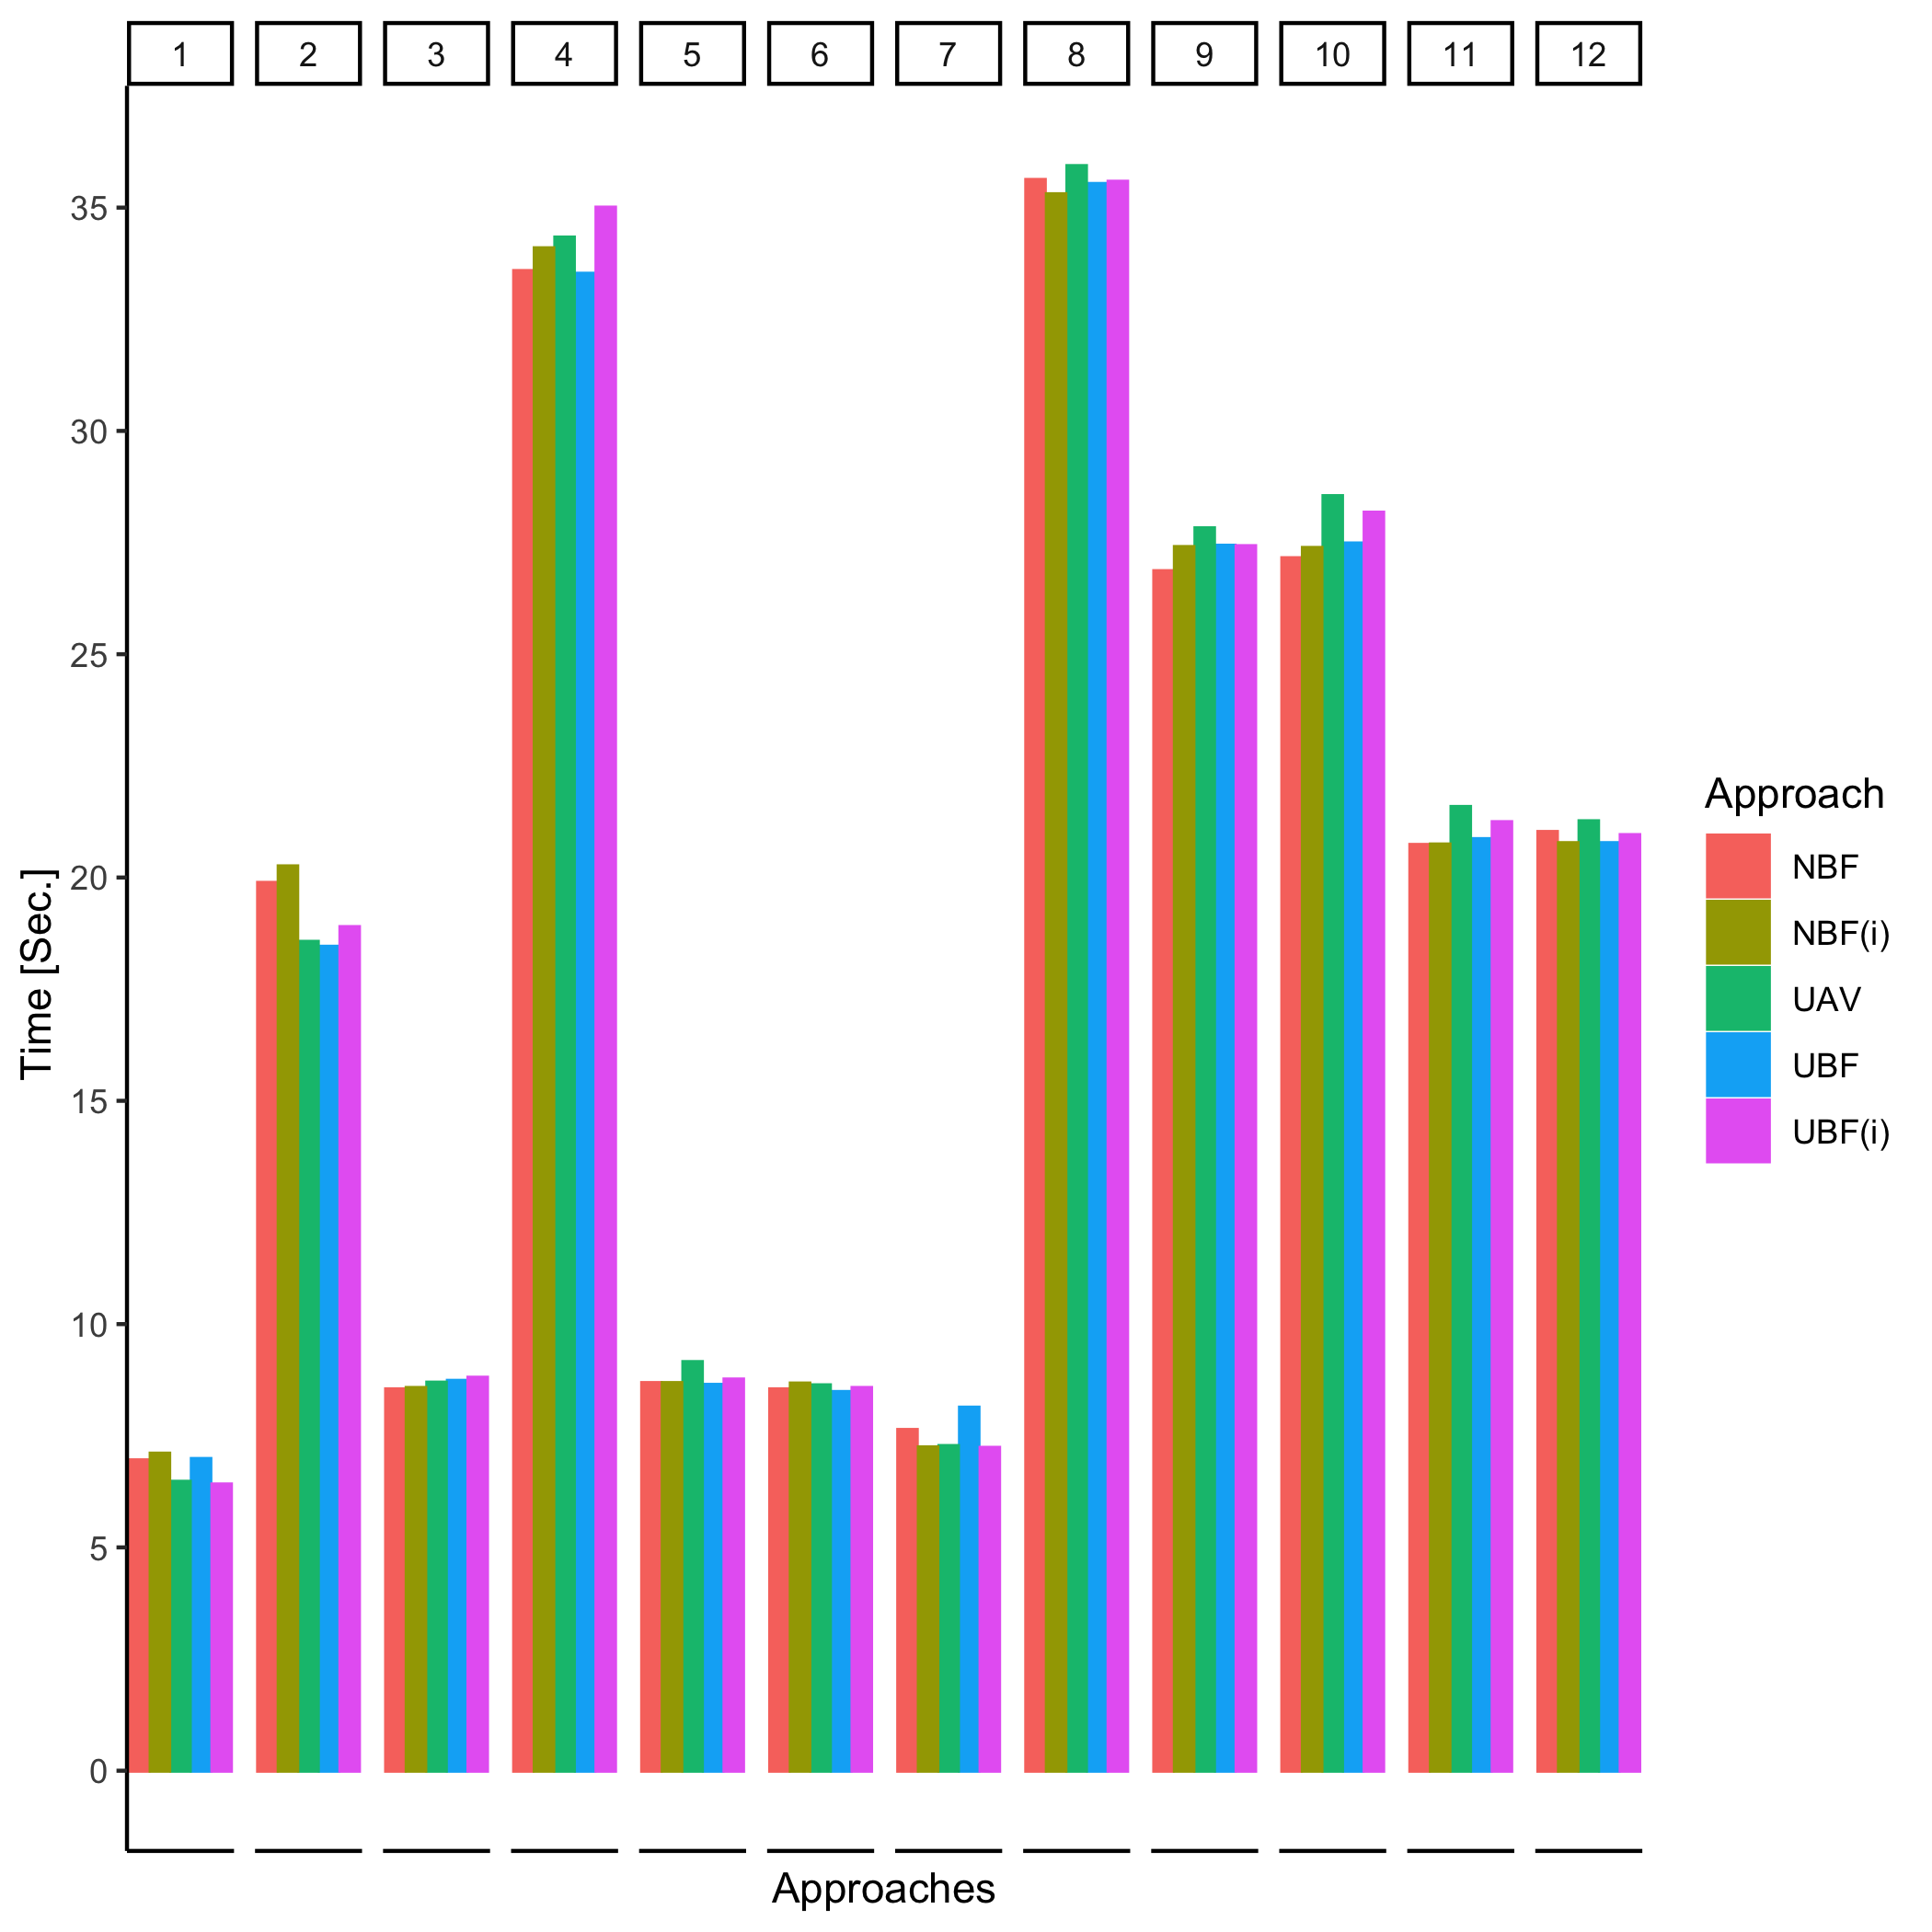
\includegraphics[scale=0.12] {figs/plots/emp1-5.png}
\caption[Comparison of SQL generators \nbf, \nbfi, \uav, \ubf, and \ubfi\ over the employee VDB]{Comparison of SQL generators \nbf, \nbfi, \uav, \ubf, and \ubfi\ over the employee VDB}
\label{fig:emp1-5}
\end{figure}



\figref{emp1-5} and \figref{enron1-5} show the runtime for each query which is shown on top the plot
for the five approaches introduced in \secref{apps} over the employee and email VDBs, respectively.
%
\figref{emp1-5} implies that  \nbf\ mostly has a better
runtime than \nbfi\ and similarly \ubf\ mostly has a better runtime than \ubfi\ for this data set. However, 
\nbf, \uav, and \ubf\ have a close performance to each other but neither consistently performs 
better than the others. 
%
%Since the most of the variational queries of the employee VDB return a small table, showed in \figref{},
%this dataset provides us with little insight. Still, \figref{emp1-5} shows that \nbf\ mostly has a better
%runtime than \nbfi\ and similarly \ubf\ mostly has a better runtime than \ubfi. This insight is confirmed 
%by \figref{enron1-5} which shows the runtime of the email VDB's queries. 
%
\figref{enron1-5} also implies that \nbf\ consistently has a better
runtime than \nbfi\ and \ubf\ mostly has a better runtime than \ubfi\ for this data set. And while
\uav\ mostly performs better than \nbf\ it is mainly comparable to \ubf\ for this data set. Yet, \uav\
sometimes generates a non-runnable SQL query, showed by the striped bars in \figref{enron1-5}.
\exref{uav-fail} explains this in detail. 


\begin{figure}[!t]
\centering
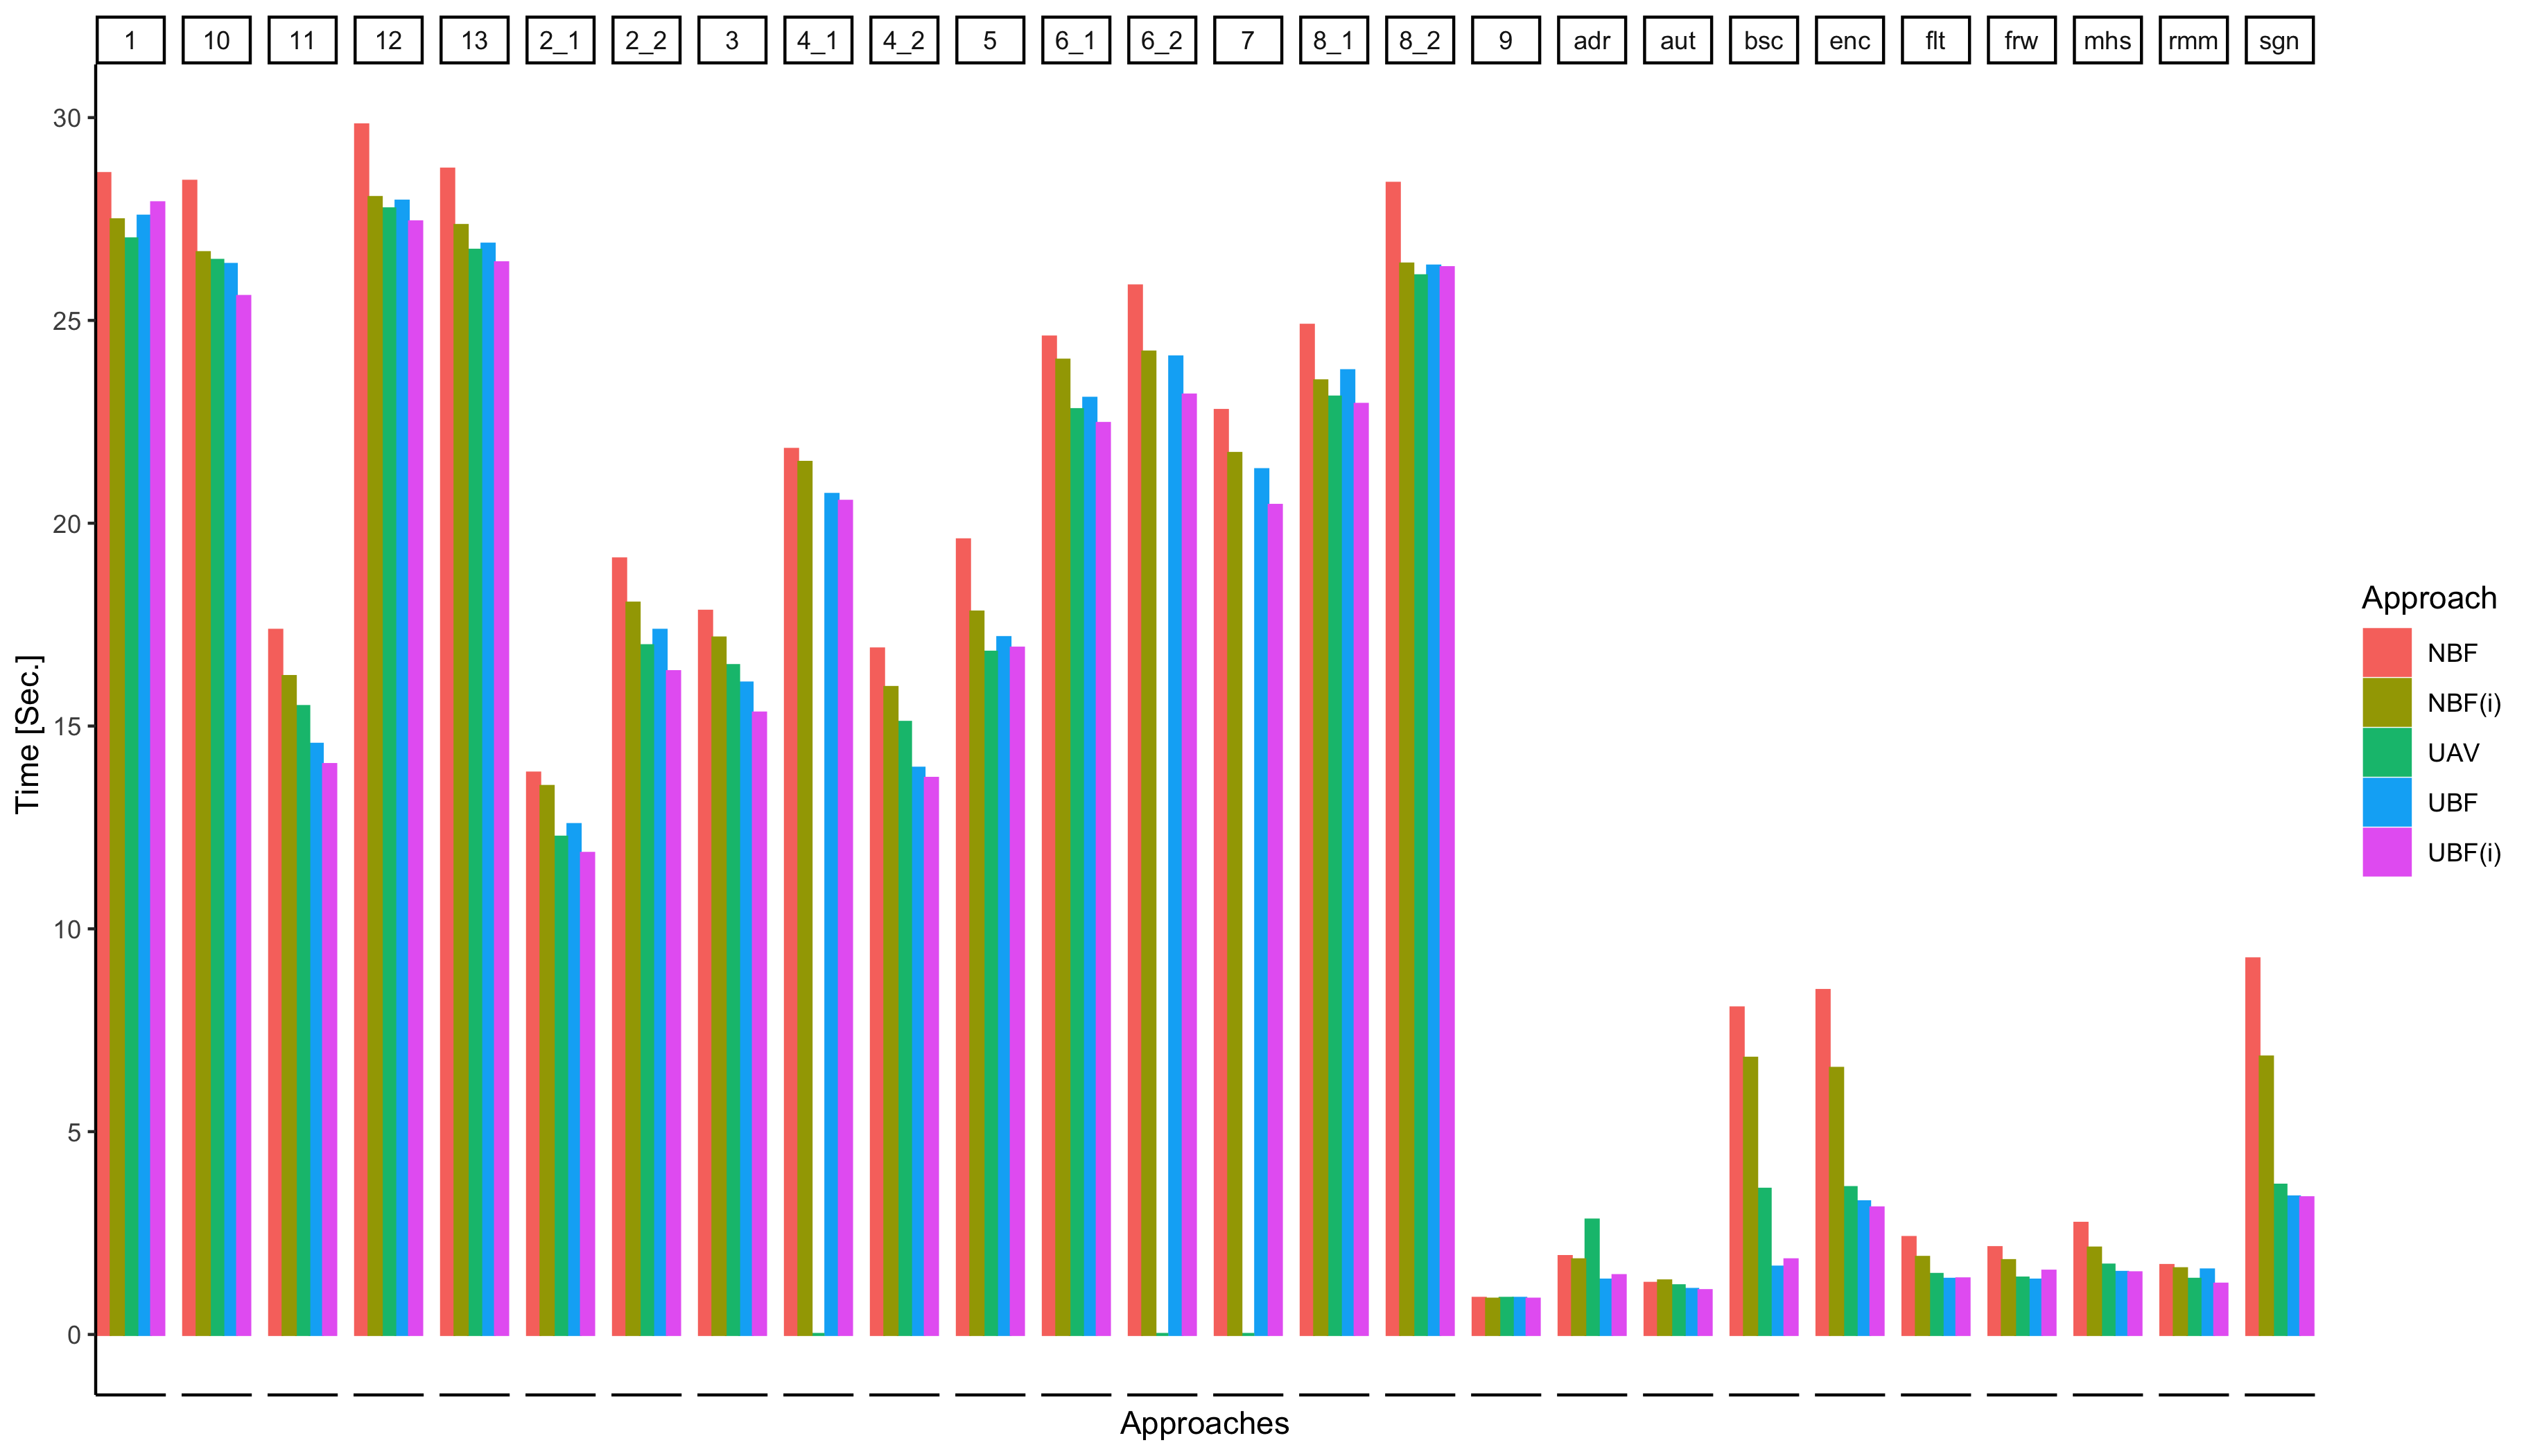
\includegraphics[width = \linewidth] {figs/plots/enron1-5.png}
\caption[Comparison of SQL generators \nbf, \nbfi, \uav, \ubf, and \ubfi\ over the email VDB]{Comparison of SQL generators \nbf, \nbfi, \uav, \ubf, and \ubfi\ over the email VDB}
\label{fig:enron1-5}
\end{figure}


%
Based on our experiments, the query construction (from type system to generating SQL queries) takes
similar time between the approaches. Their main difference comes down to the gross runtime
of queries on the VDB and building the returning variational table. 
%
\uav\ does not take any time to build a variational table since the result already have the
desired schema and presence conditions, however, it spends more time on running the 
SQL query since queries generated by \uav\ are usually more complicated. 
%
On the other hand, although \nbf\ and \ubf\ run multiple SQL queries per variational query
their generated SQL queries are simpler than the ones generated by \uav. However,
as opposed to \uav\ they have to adjust the returned table for each SQL query and apply
the correct presence condition to the tuples. 
%
Finally, the main difference between the performance of  \nbf\ and \nbfi\ (and similarly, \ubf\ and \ubfi)
is where they apply the correct presence condition to the tuples. While \nbfi\ and \ubfi\ pass this
task to the underlying database engine the \nbf\ and \ubf\ approaches load this to the Haskell 
backend. Note that all four of these approaches still have to fix the schema of the returned
tables to the variational table schema of the variational query. 

\begin{example}
\label{eg:uav-fail}
In this example we explain the reason why the SQL query generated by the \uav\ approach
sometimes cannot be run. PostgreSQL forces the type of an attribute \vAtt\ that is projected as \nul\
(that is, \texttt{NULL as \vAtt}) to be a string. Thus, using the union operation between 
subqueries when \vAtt\ has a different type causes an error. Assume the following query is 
generated by the \uav\ approach:
%
\begin{lstlisting}[basicstyle=\footnotesize\ttfamily,columns=flexible,lineskip=0.5\baselineskip]
(SELECT body,
         NULL AS is_encrypted
 FROM messages)
UNION ALL
(SELECT body,
         is_encrypted
 FROM messages)
\end{lstlisting}
%
PostgreSQL forces \isencrypted\ to have the type string while in the second subquery it assumes the boolean 
type for \isencrypted\ since that is its defined type in the  database. This causes a conflict in the assumption
that subqueries of a query that uses the union operation must have the same schema and their 
attributes must have the same type.
\end{example}

\secref{exp-vars} sheds light on the impact of number of (unique) variants on each approach and
\secref{exp-tuples} explores the effect of the number of returned tuples on our approaches. 

